%导言区
\documentclass{article}

\usepackage{ctex}
\usepackage{graphicx}

\graphicspath{{figures/}}
%正文区(文稿区)
\begin{document}
	\tableofcontents

	\section{设计背景}
	\subsection{任务阐述}
	\subsubsection{题目背景}
		数据链路层中分两个子层:介质访问控制层(MAC)和逻辑链路控制层(LLC). LLC 层是给高层提供接口并执行流量控制和差错控制的,MAC层主要负责寻址,差错检测以及介质访问控制,LLC 层在上面,MAC 在下面。介质访问控制是指将传输介质带宽有效分配给网上各站点用户的方法。\par
		如图\ref{fig-1}  所示,在有线局域网中多个主机共享一个线路的情况叫做复用,在此时如果多个主机在同一时刻访问这条线路,则主机与主机之间会产生冲突,这就是竞争。\par
		那么对于这类的竞争信道,对于任何一个主机,我们应该重点考虑三个问题:\par
		第一,	什么时候可以访问信道?这涉及到访问时机的问题;\par
		第二,冲突的检测。因为冲突是很难避免的,必须有必要措施能检测到冲突,这对于进一步处理这个冲突是必要的;\par
		第三,冲突处理。冲突之后应该怎么去处理这个冲突?这都是协议应该考虑的问题。
		此时 ALOHA 协议应用而生。ALOHA 协议是以 70 年代夏威夷通信系统为雏形,当时夏威夷大学的研究人员希望把偏僻岛屿上面的用户连接到檀香山的主计算机上面,但是就会产生上文所说的那种冲突。于是他们设计了一个 ALOHA 系统,也就是现在 ALOHA 协议的模型。
		\\
		\begin{figure}[htbp]
				\centering
				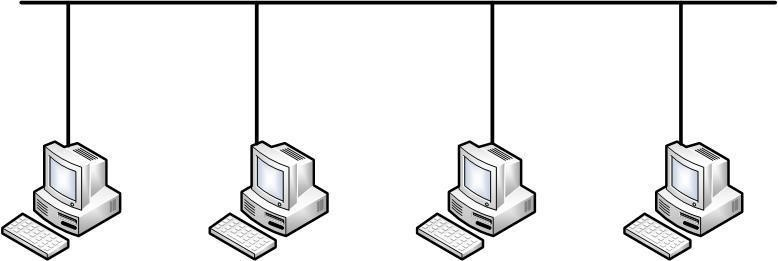
\includegraphics[scale=0.5]{1}
				\caption{链路复用}
				\label{fig-1}
		\end{figure}
	
	\subsubsection{题目内容}
	熟悉 CSMA、ALOHA 或者 CSMA/CA 协议,采用 Matlab 或者 C 语言编写程序,对其中一种自由竞争接入协议在随机布点、不同节点数、不同覆盖范围和不同退避机制等条件下进行网络性能分析。
	
	基于协议的难度,本文选择 ALOHA 协议进行仿真并分析其性能。
	
	\subsubsection{题目要求}
	1)节点数为 10-100 个以 10 个递增数量;\par
	2)网络面积为 10*10(单位平方),覆盖范围从 1-20 递增;\par
	3)画出网络容量(网络吞吐量)与各参数的变化曲线来分析网络参数对性能的影响;
	
	\subsection{任务分析}
	\subsubsection{ALOHA}
	ALOHA 协议或称 ALOHA 技术、ALOHA 网,是世界上最早的无线电计算机通信网。ALOHA协议是由美国夏威夷大学开发的一种网络协议,处于 OSI 模型中的数据链路层,是一种随机存取协议(Random Access Protocol)。它分为纯 ALOHA 协议和时隙 ALOHA 协议。
	\\ 	\par
	1.2.1.1 纯 ALOHA 协议(Pure ALOHA)\\
	\par
	纯 ALOHA 协议的实现过程\\
	1.当标签进入阅读器产生的磁场区域后,通过天线接收到电磁波而被激活,激活后的标签主动向阅读器发送消息,发送不受时间的先后限制;\\
	2.如果阅读器成功收到数据包,则会向标签发送 ACK;\\
	3.如果接收的数据包有错误,阅读器会向标签发送 NACK;\\
	4.当信道中的两个标签同时传输数据的时候,由于信道的限制和某些因素产生了数据间的碰撞会发生冲突。这种情况下,阅读器会发送一指令命令所有标签延迟发送数据。\\
	5.由于标签发送数据时间的随机性和延迟时间的随机性,使得信道内标签的数据呈现三种形式,即完成碰撞、部分碰撞和成功识别。如图\ref{fig-2}所示为纯 ALOHA算法的碰撞原理图。\\
	6.阅读器识别范围内有三个标签,当标签 1  和标签 2 发生碰撞后,阅读器命令他们随机延迟一段时间后再发送消息,直到阅读器检测出只有一个标签 3 与其通信,则成功识别出该标签。
	
	\begin{figure}[htbp]
		\centering
		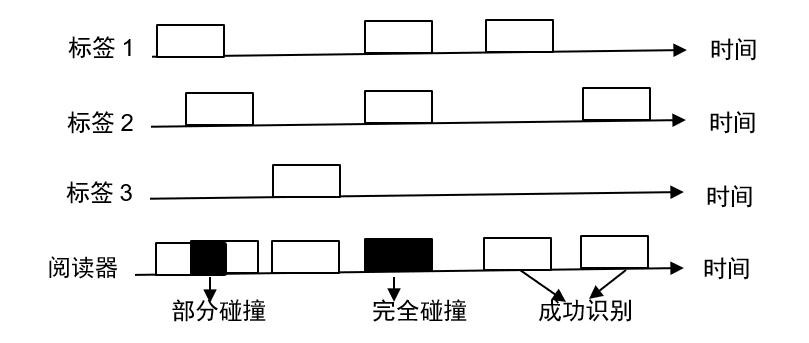
\includegraphics[scale=0.5]{2}
		\caption{ALOHA算法碰撞模型}
		\label{fig-2}
	\end{figure}
	
	\par
	1.2.1.2时隙 ALOHA 协议(Slotted ALOHA)\\
	时隙 ALOHA 实现过程\\
	1.读写器先发送 Query 指令规定帧长(时隙的个数);\\
	2.标签在帧长范围内随机地选择一个时隙响应读写器的指令并返回信息包,仅有一个标签返回信息包的时隙称为成功时隙 1,没有标签返回信息包的时隙称为空时隙 0,有 2 个或多个标签返回信息包的时隙称为碰撞时隙 ,发生碰撞的标签会在下一帧继续尝试;\\
	3.算法先根据前一帧的反馈(即观测值:碰撞时隙数量 ,空时隙 0和成功时隙1),采用一定的标签估计方法来估算场区内的标签数量 n,并且据此选择一个合适的帧长度;\\
	4.读写器以这个合适的帧长作为下一轮识别的帧长,直到读写器工作场区内的标签被全部识别完毕。\\
	本文选择纯 ALOHA 协议进行分析并仿真,故下文只提及纯 ALOHA。
	
	
	\subsubsection{ALOHA协议机制}
	Aloha协议在发送节点有数据分组发送时,节点便立即发送数据分组,启动定时器(定时的时间值为数据分组在信道中传播的一个最大来回时延值),等待目的节点发回 Acknowledge(ACK)信号,以确认数据分组被成功接收。如果发送节点在定时器的定时时间内成功接收了 ACK 信号,那么在有数据分组发送时继续发送数据分组;如果发送节点未能接受 ACK 信号,那么递增重传次数并重传数据分组,当重传次数超过预先设置的重传数据分组次数的门限值时,认为数据链路失效而放弃本次数据分组的传输。
	\subsubsection{ALOHA协议状态}
	依据 Aloha 协议的工作机制,可以得出协议工作的状态转移过程,如表\ref{table-1}所示
	\begin{table}[htbp]
		\centering
		\caption{ALOHA协议状态表}
		\label{table-1}
		\begin{tabular}{|c| c| c| c|}
			%\multicolumn{2}{空闲状态(状态 0)}
			\hline
			当前状态 & 逻辑事件 & 采取动作 & 下一状态\\
			\hline
			 1& 数据分组到达 & 发送数据分组,启动定时器 & 状态 1\\
			\hline 
			1 & 接收到数据分组 & 发送ACK  & 状态 0\\
			\hline
			2 & 接收到ACK分组 & 不采取动作(成功) & 状态 0 \\
			\hline
			2 & 定时器定时时间到 & 重发次数内则重发数据 & 状态0 \\
			\hline
			2 & 定时器定时时间到 & 已到重发次数则不采取动作 & 状态0 \\
			\hline
		\end{tabular}
	\end{table}
	\subsubsection{任务分析}
	1.	查阅资料。分析题目,查阅相关文献;\\
	2.	制定仿真计划。根据老师的要求找到一篇合适的 SCI 文献以及一篇 EI 文献,并根据 EI 文献进行仿真设计;\\
	3.	编程仿真。利用 matlab 对本课题进行仿真,仿真思路如下:\\
	a)	分模块进行仿真,首先实现在一个 10*10 的范围内进行随机布点;其次确定每个节点能与哪些节点通信,确定每个信道中的节点以及节点个数;最后在每个时刻对每个节点进行状态分析以及确定节点的状态转变; \\
	b)	对每个节点进行状态分析以及确定状态。所有节点只能有表 1 中的两种状态,并且ALOHA 协议就是让节点在这两个状态间进行转变,然后得到所有节点的发送包的成功率;\\
	c)	计算吞吐量,做节点范围-吞吐量图。
	
	\subsection{课程设计进度表}
	课程设计进度含有计划时间与实际进度时间,具体见表\ref{table-2}
	\begin{table}[htbp]
		\centering
		\caption{课程设计进度表}
		\label{table-2}
		\begin{tabular}{|c|c|c|c|}
		\hline 
		序号 & 各阶段完成的内容 & 计划时间 & 完成时间\\
		\hline
		1 & 查阅相关文献资料、课题调研 &	2018.05.04 & 2018.5.3-2018.5.7 \\
		\hline
		2 & 掌握设计软件、制订进度计划 & 2018.05.05 & 2018.5.8-2018.5.10\\
		\hline
		3 & 系统方案论证 & 2018.05.06 & 2018.5.11-2018.5.17\\
		\hline
		4 & 系统仿真各部分参数设计 & 2018.05.07 & 2018.5.18-2018.6.07\\
		\hline
		5 & 系统仿真测试及性能分析 & 2018.05.08 & 2018.6.08-2018.6.21\\
		\hline
		6 & 仿真结果检查 & 2018.05.09	 & 2018.6.26\\
		\hline
		7 & 系统完善,设计修正 & 2018.05.10 & 2018.6.27-2018.6.30\\
		\hline
		8 & 撰写课程设计说明书 & 2018.05.11  &  2018.6.31-2018.7.12\\
		\hline
		\end{tabular}
	\end{table}
	
	\section{设计方案}
	在了解了 ALOHA 协议的基础上,为进行本次课设的仿真工作,本人做了两个方案进行分析,下面一一介绍两个方案。\\
	方案一:\\
	在完成初始化工作以及随机布点工作后,将 ALOHA 协议分成以下几个状态:\\
	状态 0:空闲,节点处于空闲状态,无数据发送或者接收\\
	状态 1:发送,节点的数据分组到达则发送包\\
	状态 2:接收,节点检测到有节点在给自己发送包,则接收\\
	状态 3:发送 ACK,节点接收到其他节点发送的包后发送 ACK 表示确认收到包\\
	状态 4:接收 ACK,节点在发送完包后,则等待 ACK,如果接收到 ACK,则通信成功\\
	状态 5:重发,当信道冲突时,节点需要重发当前的包按照如图\ref{fig-3}所示的状态转变图进行状态转变。
	\\
		\begin{figure}[htbp]
			\centering
			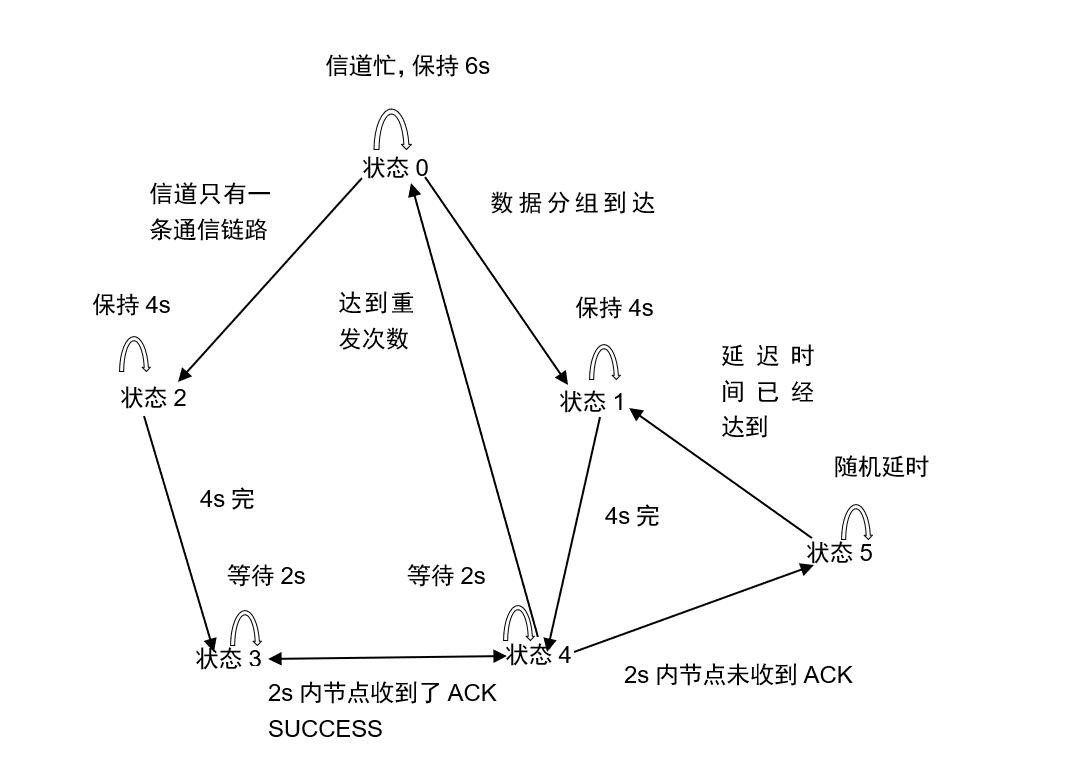
\includegraphics[scale=0.5]{3}
			\caption{方案一状态转换图}
			\label{fig-3}
		\end{figure}
	\par
	方案优缺点:\\
	优点:将通信过程分成了多个明确的状态,简单明确;\\
	缺点:从状态 0 转到状态 2 时不符合实际需求,不存在当一个节点在接收或者发送包的时候会影响其他的节点保持不变的情况。\\
	
	方案二:\\
	基于方案一,提取了更少的状态,将其他可以合并的状态转变成从一个状态转成另一个状态的逻辑条件。在本方案中将 ALOHA 协议分成两个状态:\\
	状态 0:空闲,节点处于空闲状态,无数据发送或者接收\\
	状态 1:等待 ACK 状态,节点发送完数据包后则等待 ACK\\ \par

	
	状态转变条件:\\
	第一个时刻:如果当前节点的数据分组到了,则随机选择通信节点;如果该通信节点在通信范围内,则由状态 0 转成状态 1,等待 ACK,并启动定时器;否则丢包,等待当前节点发送下一个包的时刻,状态仍然保持状态 0;\\
	状态 0-状态 1:\\
	如果当前节点不是重发,则判断是否数据分组到了;如果是则发送包,并随机选择通信节点;如果能通信则由状态 0 转成状态 1,等待ACK,并启动定时器;否则丢包,等待当前节点发送下一个包的时刻,状态仍然保持状态 0;如果数据分组未到,则判断当前是否有节点在等待自己的 ACK,并且有且仅有 1 个连续 4 个时刻都在等待此节点的 ACK,则发送 ACK;否则不做处理,继保持状态 0;\\
	如果当前节点是重发,当重发时刻到,则进入状态 1,等待 ACK;当重发时刻未到,则判断当前是否有节点在等待自己的 ACK,并且有且仅有 1 个连续 4 个时刻都在等待此节点的 ACK,则发送 ACK;否则不做处理,继保持状态 0;\\
	状态 1-状态 0:\\
	如果 10 个时刻内收到 ACK,则当前包发送接收成功,success+1,并且等待当前节点下一个包发送的时刻到来;\\
	如果 10个时刻后仍然没有ACK,则判断当前节点的重发次数有没有超过规定的数字,若没超过,则转变成状态 0,并且等待重发的时刻;若已经超过,则丢包,且转成状态 1,等待当前节点下一个包发送的时刻到来;\\
	
	方案二相对于方案一更好,方案二状态更少,并且也能清晰地描述通信过程;但是存在有某个状态未能考虑到。但总体而言,方案二更好,故本次课设选择方案二。
	
	

	
	\subsection{系统方案设计}
	\subsection{模块功能设计}
	\subsubsection{初始化参数}
	\subsubsection{随机布点及通信范围}
	\subsubsection{信道节点检测和状态转变}
	
	\section{系统仿真分析}
	\subsection{系统仿真及性能分析}
	\subsection{仿真中出现的问题及解决方法}
	\section{结果与结论}
	\section{收获与感谢}
	\section{参考文献}
	\section{附件1:问题回答记录表}
	\section{附件2:课程设计毕业要求指标点自评表}
	\section{课程设计成绩表}
\end{document}